\documentclass[a4paper,12pt]{article} %style de document
\usepackage[utf8]{inputenc} %encodage des caractères
\usepackage[french]{babel} %paquet de langue français
\usepackage[T1]{fontenc} %encodage de la police
\usepackage[top=2cm,bottom=2cm,left=2cm,right=2cm]{geometry} %marges
\usepackage{graphicx} %affichage des images
\usepackage{amssymb}
\usepackage{url}
\usepackage{verbatim}
\usepackage{amsmath}
\usepackage{color}
\usepackage{tikz}
\usepackage{hyperref}
\hypersetup{
	hidelinks,
    colorlinks,
    citecolor=black,
    filecolor=black,
    linkcolor=black,
    urlcolor=black
}

\begin{document} %début du document

%----------------------------------
%page de garde
%----------------------------------

\begin{titlepage}

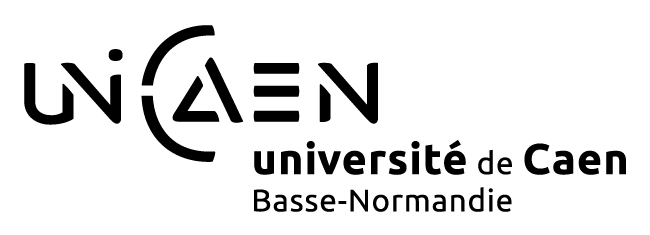
\includegraphics[scale=0.3]{images/unicaen.png}

\vspace{7cm}

\begin{center}

\begin{Huge}
TPA\\
Rapport de Projet\\
\end{Huge}
\vspace{2cm}
\begin{large}
Beauchamp Aymeric 21301016\\
Chagneux Dimitri 21606807\\
Mori Baptiste 21602052\\
Leblond Valentin 21609038\\
\vspace{1cm}
L2-Info-groupe-4A
\end{large}

\end{center}
\end{titlepage}


%------------------------------
%sommaire
%------------------------------

\newpage

\tableofcontents

\newpage

%------------------------------
%contenu
%------------------------------


\section*{Objectifs}
\addcontentsline{toc}{section}{Objectifs}

\subsection*{Description du Sokoban}
\addcontentsline{toc}{subsection}{Description du Sokoban}

Le Sokoban est un jeu de réflexion de type puzzle où le joueur doit placer des caisses sur des objectifs placés à l'avance sur la carte. Le joueur gagne si toutes les caisses sont placées sur les objectifs et il ne peut pousser qu'une seule caisse à la fois. Il existe de nombreux niveaux dont la difficulté est variable.

\begin{figure}[!h]
\centering
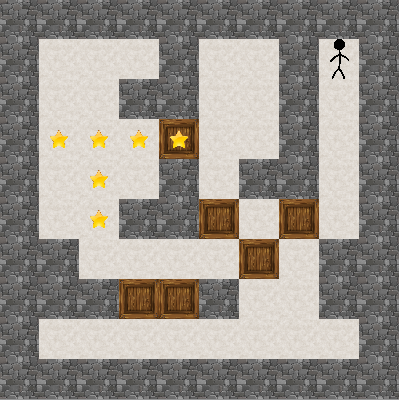
\includegraphics[scale=0.5]{images/sokoban.png}
\caption{Niveau de Sokoban}
\end{figure}

\subsection*{Les fonctionnalités attendues}
\addcontentsline{toc}{subsection}{Les fonctionnalités attendues}

Pour ce projet, nous devions mettre au point une version jouable pour un humain en console, en prenant en compte l'importation de niveaux (au format \textbf{.xsb}). Il était également demandé de réaliser une interface graphique et une fonctionnalité permettant une résolution automatique de niveau.\\
Enfin, permettre de faire jouer en parallèle un humain et un ordinateur, et rendre \textit{anytime} l'algorithme de l'intelligence artificielle. C'est à dire le fait que lorsque le joueur fait un mouvement, l'intelligence artificielle doit en faire un.


\section{Fonctionnalités implémentées}

\subsection{Description des fonctionnalités}

\subsubsection*{Attendues}
\addcontentsline{toc}{subsubsection}{Attendues}

La version console fonctionne à l'aide de saisies de l'utilisateur qui lui permettent de contrôler le jeu. Une fois un niveau terminé, on demande au joueur si il souhaite passer au niveau suivant.\\

La carte est chargée à partir d'un fichier \textbf{.xsb} contenant des lignes de caractères, que l'on transforment en liste de caractères.\\
La carte est donc modélisée par des chaînes de caractères:
\begin{itemize}
\item \textbf{\#} pour un mur
\item \textbf{\$} pour une caisse
\item \textbf{@} pour le joueur
\item \textbf{.} pour un objectif
\item \textbf{*} pour une caisse sur un objectif
\item \textbf{+} pour le joueur sur un objectif
\item \textbf{espace} pour les cases vides
\end{itemize}

\begin{figure}[!h]
\centering
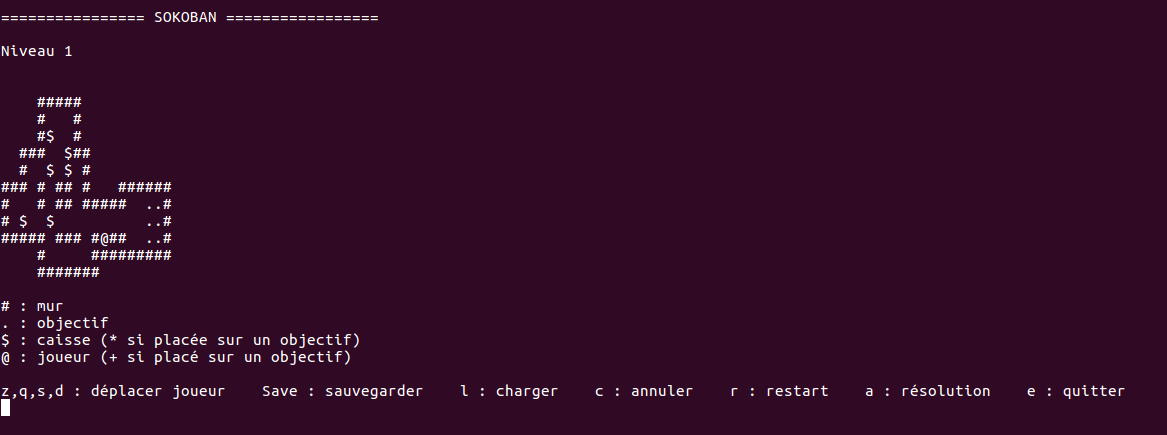
\includegraphics[scale=0.5]{images/Capture.png}
\caption{Interface console}
\end{figure}

Au niveau de l'interface graphique, nous avons une zone de jeu dans laquelle on dessine le niveau et des boutons pour gérer les différentes fonctionnalités. Le personnage est déplaçable avec les flèches directionnelles ou ZQSD, si le joueur a bloqué une caisse ou si il a gagné, il ne peut plus bouger et doit recommencer le niveau ou passer au suivant (seulement si il a gagné). Si le joueur gagne, le personnage effectue le Dab et si il perd, le personnage pleure.\\

Il est possible de demander la résolution automatique du niveau. Un solveur calcule alors un itinéraire permettant de ranger toutes les caisses à partir de la position du joueur.

On peut également jouer contre l'IA en simultané.

\begin{figure}[!h]
\centering
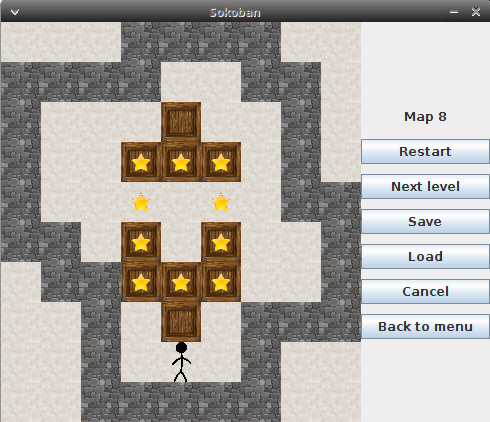
\includegraphics[scale=0.5]{images/Capture2.png}
\caption{Interface graphique}
\end{figure}

\subsubsection*{Ajoutées}
\addcontentsline{toc}{subsubsection}{Ajoutées}

Au lancement du programme, l'utilisateur peut choisir un profil ou en créer un nouveau.\\
En fonction de l'avancement du profil donné, le joueur a débloqué un certain nombre de cartes ; pour débloquer la carte suivante il faut finir le niveau en cours. Lorsqu'un profil est chargé, la dernière carte non terminée est lancée automatiquement.\\

Nous proposons également à l'utilisateur de sauvegarder sa partie à un instant du niveau donné, de charger sa sauvegarde (il n'y a pas de conflit entre les sauvegardes des différents utilisateurs), d'annuler le dernier coup joué  et enfin de recommencer le niveau courant.

\subsection{Organisation du projet}

Pour le début du projet, nous avons tous travaillé sur la conception du modèle du jeu : comment représenter chaque élément qui compose le jeu (joueur, case vide, caisse ou encore la carte qui les contiendra). Ensuite nous nous sommes interrogés sur la manière de déplacer le joueur ainsi que faire pousser les caisses par le joueur et faire en sorte de gérer les collisions avec les murs.\\
Nous avons rencontrés des difficultés pour la détection d'une caisse bloquée. Nous nous sommes d'abord contentés de considérer le cas où une caisse est bloquée par deux murs de telle façon qu'il est impossible de la déplacer (cas de gauche de la \textbf{figure \ref{figure4}}).\\
Nous nous sommes vite rendus compte que ce n'était pas le seul cas de caisse bloquée, comme on peut le voir sur la deuxième image de la \textbf{figure \ref{figure4}}. En effet, on ne peut déplacer aucune des deux caisses car elles se bloquent entre elles. Nous avons donc gérer ce cas, mais il était loin d'être le dernier, le sokoban étant un jeu très facile à bloquer. Les cas plus complexes sont traités dans la partie \hyperref[et]{Eléments techniques}.

\begin{figure}[!h]
\centering
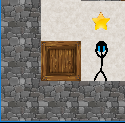
\includegraphics[scale=0.5]{images/Capture3.PNG}
\hspace{1cm}
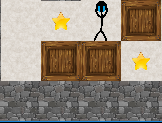
\includegraphics[scale=0.5]{images/Capture4.PNG}
\caption{Blocage simple de caisses}
\label{figure4}
\end{figure}

Ensuite, nous nous sommes séparés en trois groupes, deux d'entre nous ont débuté la conception d'une IA capable de résoudre des niveaux du jeu, et une autre personne s'est lancée dans la création de la classe principale avec interface console ainsi que toute la gestion de fichiers (sauvegarde, chargement, traduction entre une carte enregistrée dans un fichier et notre représentation d'un niveau de notre code). Le dernier membre s'est occupé de gérer les cas complexes de détections de caisses bloquées puis s'est attelé au développement de l'interface graphique.\\

L'interface graphique ayant bien avancé, des nouvelles fonctionnalités ont été ajoutées dans celle-ci (telles que la sélection de profils) et des réglages dans la manière de sauvegarder une map ont été modifiés, ce qui a posé problème : le modèle était devenu obsolète par rapport à l'interface graphique. Il a donc fallu revoir notre classe principale pour y implémenter la gestion de profils, et changer la manière de sauvegarder une map car la première version ne nous permettait pas de recommencer le niveau courant.\\

Au niveau de l'IA, nous avons d'abord conçu un système de déplacement automatique du joueur avant de concevoir un solveur. Nous avons passé beaucoup de temps sur une première implémentation techniquement fonctionnelle mais incapable de résoudre des niveaux qui ne soient pas extrêmement simples, avant de passer à une seconde implémentation bien plus efficace et utilisant les outils développés pour la première. 

\section{Éléments techniques}\label{et}

\subsection{Structures de données utilisées}

Le niveau de sokoban, une fois lu dans un fichier .xsb, est représenté avec une grille d'objets. Le principal avantage de cette méthode est l'intuitivité de la représentation.
Les positions des caisses et des objectifs sont stockées dans des listes du fait de l'importance de ces informations. Cela évite de devoir charger la grille dès qu'on a besoin d'une position.\\

Dans le package ia, nous utilisons des tables de hashage avec les algorithmes de recherche en tant que mémoire. Cela nous permet de pouvoir vérifier rapidement si un élément a déjà été vu, surtout lorsque l'on explore plusieurs centaines de milliers d'états.
Le solveur lui-même tient sa performance d'une file de priorité qui guide la recherche de la solution.

\subsection{Gestion des deadlocks}

Les caisses en deadlock (qui bloquent définitivement le jeu) ont plusieurs niveaux de test à passer avant d'être déclarées bloquées, il ne faut pas seulement regarder leur voisinage car une caisse peut ne pas pouvoir être déplacée sans que la partie soit finie pour autant.

\subsubsection{Cas du simple voisinage}

Une caisse est bloquée si elle possède deux voisins de type caisse et/ou de type mur. Dans ce cas, il est impossible de pousser cette caisse car un des deux éléments est situé derrière.\\

Cas simples de caisse bloquée (en rouge) : 

\begin{figure}[!h]
\centering
\begin{tabular}{ l c r }
\# & \textcolor{red}{\$} & \ \\
\  &      \#             & \ \\
\\
\hline
\end{tabular}

\begin{tabular}{ l c r }\\
\$ & \textcolor{red}{\$} & \ \\
\  &      \#             & \ \\
\\
\hline
\end{tabular}

\begin{tabular}{ l c r }\\
\# & \textcolor{red}{\$} & \ \\
\  &      \$             & \ \\
\\
\hline
\end{tabular}

\begin{tabular}{ l c r }\\
\$  &   \textcolor{red}{\$}  & \ \\
\   &        \$              & \ \\
\end{tabular}

\caption{Cas possibles de deadlock du point de vue d'une caisse}
\end{figure}

\subsubsection{Le cas des caisses bloquées entre elles}
\label{cBetween}

Le second cas c'est quand deux caisses se bloquent mutuellement. Dans l'exemple de la figure \ref{DL2}, la caisse de gauche à un mur sous elle et est à côté d'une caisse qui à aussi un mur dans le même axe donc elles se bloquent entre elles car on ne peut pousser aucune des deux.

\begin{figure}[!h]
\centering
\begin{tabular}{ l c r }
\textcolor{red}{\$} & \textcolor{red}{\$} \\
\#                  &     \#              \\
\end{tabular}
\caption{Formation d'un carré avec des murs}
\label{DL2}
\end{figure}

Un autre exemple de blocage mais sans murs cette fois, c'est le cas où quatre caisses forment un carré.

\begin{figure}[!h]
\centering
\begin{tabular}{ l c r }
\textcolor{red}{\$} & \textcolor{red}{\$} \\
\textcolor{red}{\$} & \textcolor{red}{\$} \\
\end{tabular}
\caption{Formation d'un carré avec des caisses}
\end{figure}

\subsubsection{Trouver un deadlock dans un état donné}

Maintenant que nous avons vu les cas possibles de deadlock, il faut maintenant les mettre en commun afin de pouvoir détecter les différents cas. Nous parcourons la liste des caisses et pour chaque caisse nous testons les cas vus précédemment. On teste d'abord si la caisse est entourée d'au moins deux murs sur chaque axe, si c'est le cas elle est forcément en deadlock.\\
Ensuite nous regardons si elle est bloquée par au plus un mur et au minimum une autre caisse sur chaque axe. Si c'est le cas, on teste si on se trouve dans le cas du \ref{cBetween}, c'est-à-dire si elle se bloque avec la caisse à côté d'elle.\\
Si la caisse est dite bloquée avec au plus un mur alors qu'elle n'a aucun mur autour d'elle, c'est donc qu'elle est bloquée entre deux caisses et ne peut pas être directement déplacée. Pour trouver ce cas, on teste si la caisse forme un carré avec quatre autres caisses ou éventuellement un mur (voir figure \ref{DLcarreMur}).

\begin{figure}[!h]
\centering
\begin{tabular}{ l c r }
\$                  & \# \\
\textcolor{red}{\$} & \$ \\
\end{tabular}
\caption{Formation d'un carré avec trois caisses et un mur}
\label{DLcarreMur}
\end{figure}

\subsubsection{Étude d'un cas complexe}

Pour cette étude, nous allons supposer avoir l'état de la figure \ref{DLCompl}. Nous pouvons voir que la caisse bleue est bloquée par la caisse verte et un mur, mais que la caisse verte peut être déplacée à gauche ou à droite pour ne plus bloquer la caisse bleue. La caisse bleue n'est donc pas en deadlock.\\
Si on continue de parcourir la liste des caisses et qu'on tombe sur une des caisses rouges, on s'aperçoit qu'elles forment un carré avec les autres caisses rouges. Nous avons trouvé un deadlock et on retourne alors l'information que le niveau ne peut pas être terminé dans l'état actuel. La caisse orange n'est pas considérée comme un deadlock malgré le fait qu'elle soit bloquée avec la caisse noire car cette dernière n'a pas de mur dans le même axe que la caisse orange et ne forme pas de carré avec des murs et/ou caisses.

\begin{figure}[!h]
\centering
\begin{tabular}{ l*{4} c*{5} r }
\# & \# & \# & \# & \# & \# & \#\\
\# & \ & \ & \ & \ & \ & \#\\
\# & \  & \  & \# & \textcolor{blue}{\$} & \ & \#\\
\# & \  & \  & \  & \textcolor{green}{\$} & \ & \#\\
\# & \  & \  & \textcolor{orange}{\$} & \$ & \ & \#\\
\# & \textcolor{red}{\$} & \textcolor{red}{\$} & \# & \ & \ & \#\\
\# & \textcolor{red}{\$} & \textcolor{red}{\$} & \  & \ & \ & \#\\
\# & \ & \ & \ & \ & \ & \#\\
\# & \# & \# & \# & \# & \# & \#\\
\end{tabular}
\caption{Exemple de cas complexe}
\label{DLCompl}
\end{figure}

\subsection{Déplacement du joueur par l'IA}\label{astar}

Pour obtenir une granularité dans le déplacement du joueur par l'IA, nous avons implémenté l'algorithme de recherche de chemin A*. On utilise des objets \textbf{Node} qui possèdent en attribut des coordonnées et un nœud prédécesseur. Pour chaque nœud, on calcule le coût du chemin entre le départ et la destination passant par ce nœud. Le coût du chemin s'exprime :

$$ f(x) = g(x) + h(x)$$

où $g(x)$ est le coût du chemin depuis le départ et $h(x)$ est une fonction heuristique estimant le coût pour atteindre la destination.\\

Le calcul de $g(x)$ consiste à compter récursivement les prédécesseurs du nœud jusqu'à arriver au départ.\\
L'heuristique utilisée pour $h(x)$ est la distance de Manhattan : la décomposition de la distance euclidienne entre deux points en une composante verticale et une composante horizontale. Cette heuristique est adaptée au Sokoban étant donné qu'on ne peut pas se déplacer en diagonale. Elle est également admissible pour A* : elle ne sous-estime jamais la distance à l'arrivée. Cela garantit que le chemin trouvé est optimal.

\begin{figure}[!h]
\centering
\begin{tikzpicture}
\node (depart) at (0,0) {A};
\node (arrivee) at (2,2) {B};
\coordinate (x) at (2,0);
\draw[color=blue] (depart) -- node[left] {Distance euclidienne}(arrivee);
\draw[color=red] (depart) -- node[below] {Distance de Manhattan} (x);
\draw[color=red] (x) -- (arrivee);
\end{tikzpicture}
\caption{Illustration de la distance de Manhattan}
\end{figure}

Le fonctionnement de cet algorithme est le suivant :\\

\begin{itemize}
\item On initialise l'algorithme avec les positions du joueur et de sa destination et on ajoute la position du joueur dans une liste d'attente. On crée aussi deux tables de hashage avec autant de clés qu'il y a de positions libres dans la grille. Les clés sont des objets Node ; à ces clés sont associées la valeur du nœud que l'on initialise à +$\infty$.
\item On retire de la liste d'attente l'élément ayant le plus faible $f(x)$ et on vérifie si il correspond à la destination. Si ce n'est pas le cas, on le met dans une liste des nœuds explorés. On calcule aussi $g(voisin)=g(en\_cours)+1$, une estimation de la distance entre les voisins et le départ.
\item On calcule les voisins du nœud. Toute case n'étant pas un mur est considérée comme un nœud dans ce calcul. On ajoute à la liste d'attente les voisins pas encore explorés.
\item Pour chaque voisin, on compare $g(voisin)$ à la valeur correspondante dans la table de hashage de \textit{g}. Si $g(voisin)$ est plus petit que la valeur stockée alors on met à jour les deux tables de hashage pour le voisin et on lui attribue le nœud courant comme prédécesseur.
\item Lors que le nœud de destination est atteint, on construit le chemin trouvé en remontant récursivement les prédécesseurs du nœud d'arrivée jusqu'au nœud de départ. On obtient ainsi la liste des nœuds composant le chemin.
\end{itemize}

\begin{figure}[!h]
\centering
\begin{tikzpicture}
\node at (0,0) {@};
\draw[color=red] (0,0) circle(0.5);
\node at (1,0) {2};
\draw (1,0) circle(0.5);
\node at (2,0) {4};
\draw (2,0) circle(0.5);
\node at (0,1) {1};
\draw[color=red] (0,1) node[left] {chemin trouvé} circle(0.5);
\node at (0,2) {3};
\draw[color=red] (0,2) circle(0.5);
\node at (1,2) {5};
\draw[color=red] (1,2) circle(0.5);
\node[draw=black] at (2,1) {\#};
\node at (2,2) {.};
\draw[color=red] (2,2) circle(0.5);
\node at (3,0) {6};
\draw (3,0) circle(0.5);
\node at (3,1) {8};
\draw (3,1) circle(0.5);
\node at (3,2) {9};
\draw (3,2) circle(0.5);
\node[draw=black] at (1,1) {\#};;
\draw[->] (0,0) -- (1,0);
\draw[->] (1,0) -- node[below] {chemin exploré} (2,0);
\draw[->] (2,0) -- (3,0);
\end{tikzpicture}
\caption{Exemple d'exécution de A* pour le déplacement}
\end{figure}

La façon dont nous avons conçu la méthode de calcul de voisins pousse l'algorithme à explorer le graphe dans le sens horaire : d'abord le voisin du haut, puis à droite, etc. Ainsi, si deux chemins équivalents existent entre deux points, celui allant le plus vers le haut du niveau sera retenu. Ce biais ne semble toutefois pas influer sur l'efficacité de la recherche.

\subsection{Solveurs}

\subsubsection{Modélisation du problème}

Le sokoban est un problème complexe à résoudre du fait de plusieurs facteurs tels que le nombre de déplacements nécessaires, la facilité à tomber dans un état bloquant ou l'ordre de rangement des caisses. Il est néanmoins possible de modéliser un état du jeu et de programmer un algorithme capable d'effectuer une recherche sur ces états pour trouver un état solution du problème.\\

Avant d'implémenter un solveur, nous avons d'abord défini ce que nous considérons comme un état du jeu. Un état est représenté par un objet Board décrivant le plateau de jeu, une liste de coups et une valeur.\\
Un coup représente la poussée d'une caisse, il est défini comme une position et une direction de poussée. La poussée est l'action la plus importante du sokoban car elle modifie la disposition du plateau : elle permet la transition entre deux états du jeu.
Nous pouvons donc nous contenter de faire une exploration d'états de poussée en poussée et non de mouvement en mouvement. Cela réduit énormément le nombre d'états à parcourir.\\
La valeur d'un état est calculée par une fonction d'évaluation heuristique. C'est elle qui permet de guider la recherche pour réduire le temps de calcul et le nombre d'états explorés. Dans le cadre de ce projet, nous avons réalisé deux fonctions heuristiques :\\
\begin{itemize}
\item La première est la somme des distances de Manhattan entre chaque caisse et l'objectif le plus proche : $$h_m= \Sigma(d_m(caisse))$$
\item La seconde est une distance de Hamming : on compte le nombre de caisses qui ne sont pas placées sur un objectif.
\end{itemize}
Dans les deux cas, on passe la valeur à +$\infty$ si l'état comporte un deadlock, et un état résolu vaut 0. Le solveur va donc chercher les états de valeur minimale.\\

\subsubsection{Première implémentation}

Le premier solveur que nous avons codé est inspiré de l'algorithme minmax. On entre un état et une profondeur de recherche, et l'algorithme compare les valeurs des états successeurs de l'état entré jusqu'à atteindre les feuilles de l'arbre de recherche. Bien entendu, on ne veut ici que minimiser la valeur puisqu'il n'y a qu'un seul joueur.

\begin{figure}[!h]
\centering
\begin{tikzpicture}
\node (dep) at (0,0) {26};
\draw[color=red] (0,0) circle(0.5);
\node (e1) at (-1.25,-2) {26};
\draw[color=red] (-1.25,-2) circle(0.5);
\node (e2) at (1.25,-2) {41};
\draw (1.25,-2) circle(0.5);
\node (e3) at (-3,-4) {33};
\draw (-3,-4) circle(0.5);
\node (e4) at (-1.5,-4) {26};
\draw[color=red] (-1.5,-4) circle(0.5);
\node (e5) at (0,-4) {54};
\draw (0,-4) circle(0.5);
\node (e6) at (2,-4) {41};
\draw (2,-4) circle(0.5);
\node (e7) at (4,-4) {42};
\draw (4,-4) circle(0.5);
\draw[color=red] (dep) -- (e1);
\draw (dep) -- (e2);
\draw (e1) -- (e3);
\draw[color=red] (e1) -- (e4);
\draw (e1) -- (e5);
\draw (e2) -- (e6);
\draw (e2) -- (e7);
\end{tikzpicture}
\caption{Illustration du fonctionnement du solveur "minmin"}
\end{figure}

Malheureusement, bien que l'algorithme fonctionne, ce solveur n'a pas permis de résoudre même des niveaux très simples avec une seule caisse.

\subsubsection{Solveur A*}

Nous avons décidé de repartir du modèle que nous avions défini pour faire un autre solveur plus simple faisant un parcours en largeur des états.
Ce second solveur commence à un état initial, génère tous les états successeurs (en essayant chaque coup disponible qui modifie la position des caisses), les mémorise puis les stocke dans une liste d'attente avant de recommencer avec le premier état de la liste jusqu'à trouver une solution.\\
Avec cette version, nous avons été capable de résoudre plusieurs niveaux en une quinzaine de secondes en moyenne.\\

Nous avons ensuite amélioré le solveur en passant du parcours en largeur à l'algorithme A* décrit en \ref{astar}. Dans les faits, nous avons remplacé la liste d'attente par une file de priorité capable de trier les états selon leur valeur. Nous avons aussi découvert que la distance de Hamming était une heuristique plus efficace que notre calcul de distances de Manhattan. Nous avons ainsi pu résoudre plus de niveaux et beaucoup plus rapidement ( de l'ordre de la seconde).\\
Cependant le solveur a de gros problèmes de mémoire : la taille de la table de hashage qui mémorise les états explorés pousse le garbage collector de Java à envoyer une OutOfMemoryError et termine prématurément le programme. Cela est causé par le nombre d'états à explorer dans des niveaux complexes et la mémoire que prend chaque état. Nous avons évalué le nombre maximal d'états stockables avant de dépasser la mémoire allouée à 190 000.
Nous avons alors essayé d'optimiser le solveur, par exemple en faisant téléporter le joueur entre les coups plutôt que de lancer une recherche de chemin A* systématique ou en empêchant les caisses en deadlock sur un objectif de générer des coups. Cela a amélioré la vitesse de résolution mais n'a pas suffi a résoudre le problème de mémoire.

\subsection{Gestion de fichiers}

Afin de faciliter la lecture et l'écriture de fichiers, nous avons codé une classe \textit{FileManagement}. Cette classe contient des méthodes permettant d'enregistrer un Board, en faisant simplement appel à une classe \textit{Save} puis à une méthode de cette classe.
Ainsi, dans le Main, nous n'avons besoin que d'une ligne pour sauvegarder.
\\

Cette classe contient également des méthodes pour charger une sauvegarde, ou pour charger un fichier cancel (fichier que l'on charge lorsque l'utilisateur décide de revenir un coup en arrière). Pour ce faire nous faisons simplement appel aux méthodes de la classe \textit{MapReader}
\\

Lorsque l'on sauvegarde un Board, qui est une grille de \textit{Block}, dans un fichier, on transforme la grille en liste de String dans laquelle chaque type de Block a un caractère associé. On obtient donc une liste de String où chaque élément correspond à une sous-liste de notre grille.\\

Ensuite on fait appel à une méthode de \textit{FileManagement} en lui passant en paramètre la liste créée. Cette méthode fera appel à une méthode de \textit{Save}. Cette dernière parcourt la liste de String créée précédemment et pour chaque String on l'ajoute à une variable temporaire, que l'on écrira ensuite dans le fichier.

\section{Architecture du projet}

\subsection{Organisation des packages}

Notre projet se décompose en trois packages distincts:
\begin{itemize}
\item le package \textbf{sokoban}, le package principal contenant le modèle du sokoban, et la gestion de fichier, utilisé dans les deux autres packages;
\item le package \textbf{graphique}, qui gère l'interface graphique;
\item le package \textbf{ia}, qui implémente les algorithmes de résolution automatique.
\end{itemize}

En créant ces trois packages, nous avons pu travailler en parallèle sur différents aspects du projet sans pour autant se gêner les uns les autres.
Ainsi, une modification du package \textbf{ia} ne changeait rien au fonctionnement du sokoban en version console ou graphique.\\
Cependant, après modification du package \textbf{sokoban}, tout le groupe devait récupérer la version la plus récente, car ce package est utilisé par les deux autres puisqu'il contient le modèle.

\begin{figure}[!h]
\centering
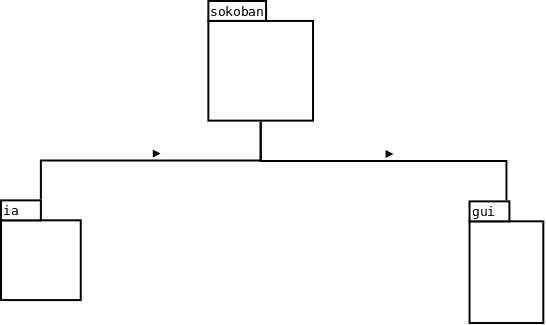
\includegraphics[scale=0.3]{images/packages.png}
\caption{Diagramme du projet}
\end{figure}

\subsection{Organisation des classes}

\subsubsection{Package sokoban}

Notre package principal comporte treize classes réparties en différentes catégories:
\begin{itemize}
\item les classes gérant les entités (personnage, murs, ...);
\item les classes permettant d'enregistrer/charger une sauvegarde;
\item les classes permettant de lancer le programme.
\end{itemize}

Toutes les classes de gestion des entités héritent de la classe \textit{Block}, elles permettent de déplacer facilement le personnage et les caisses, de gérer les collisions, les blocages et la fin d'une partie.

Les classes gérant les fichiers permettent de lire et d'écrire dans des fichiers situés dans un dossier "maps" contenant toutes les cartes du jeu, ou dans un fichier "save" stockant les profils et leur sauvegarde/cancel.

Les classes permettant de lancer le programme sont le Board, qui créer la grille de jeu, et le Main.

\begin{figure}[!h]
\centering
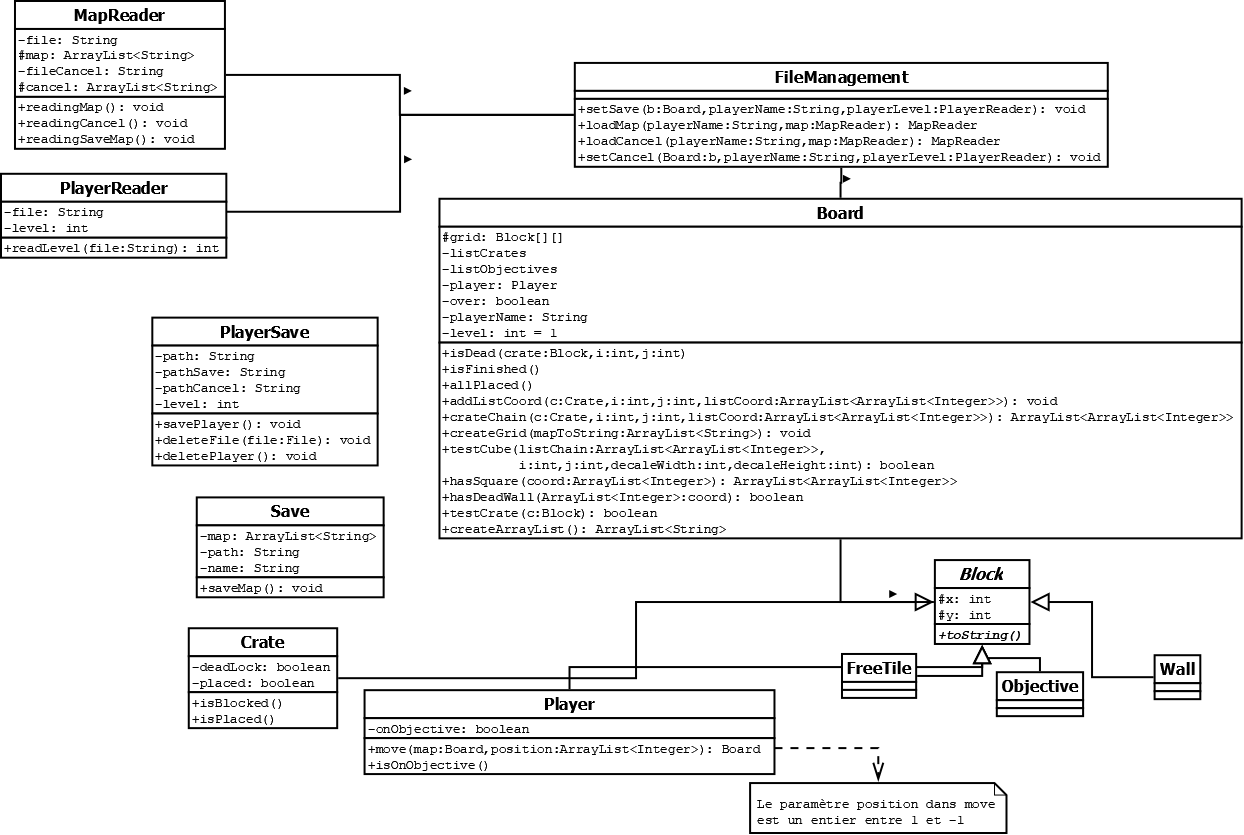
\includegraphics[scale=0.3]{images/diag_sokoban.png}
\caption{Diagramme du package sokoban}
\end{figure}

\subsubsection{Package graphique}

Ce package permet simplement de gérer la version graphique du Sokoban et de jouer sans les entrées claviers (en appuyant directement sur une touche, on peut déplacer le joueur).

\begin{figure}[!h]
\centering
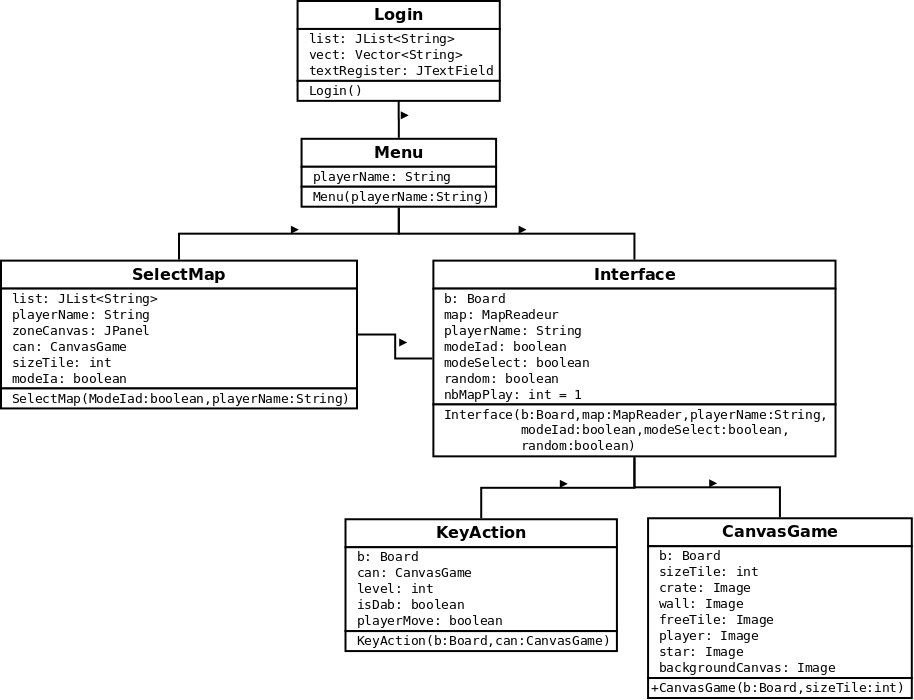
\includegraphics[scale=0.4]{images/graphique.png}
\caption{Diagramme du package graphique}
\end{figure}

\subsubsection{Package ia}

Ce package contient tout ce qui a trait à la résolution automatique du jeu. On y trouve des classes modélisant des concepts liés au jeu, et des classes contenant les algorithmes de recherche.

\begin{figure}[!h]
\centering
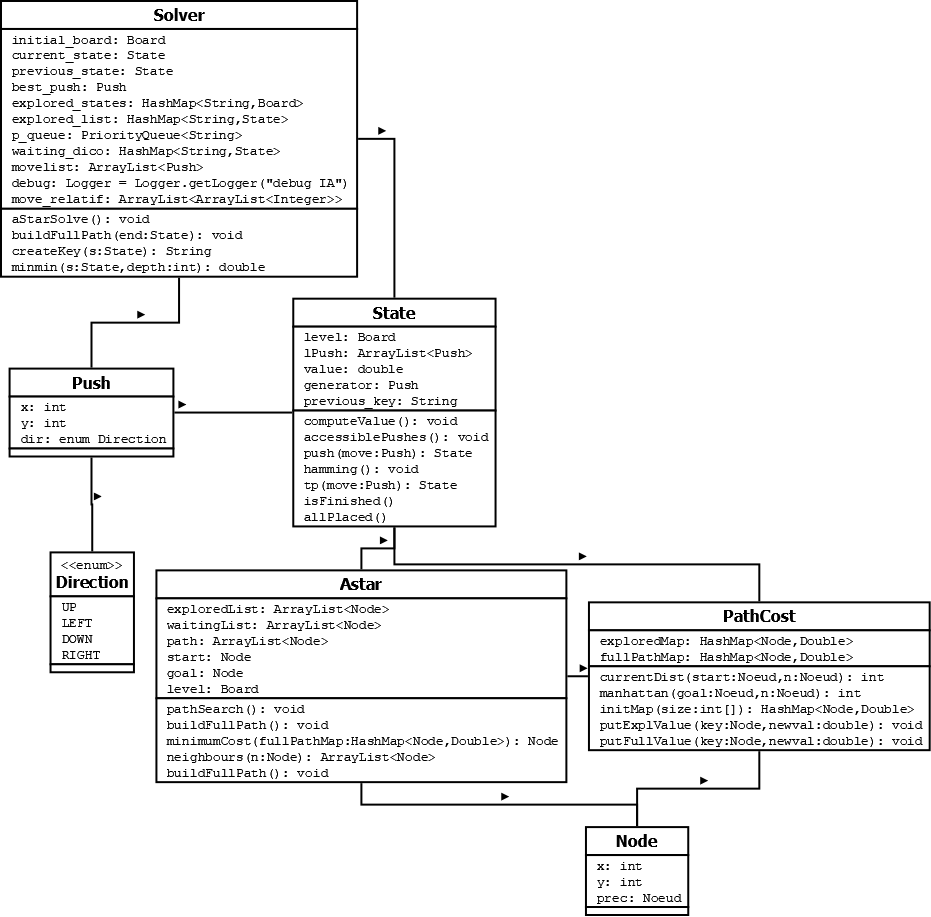
\includegraphics[scale=0.3]{images/diag_ia.png}
\caption{Diagramme du package ia}
\end{figure}

\section{Expérimentations et usages}

\subsection{Performance du solveur}

Sur la série de niveaux originaux de Sokoban, le solveur n'est capable de résoudre que le premier, en 1,5 secondes. Les autres causent des dépassements mémoire. Cela dit, les niveaux originaux deviennent vite grands, complexes, et comportent de nombreuses caisses. Notre solveur étant plutôt simple, il n'est donc pas surprenant qu'il ne parvienne pas  résoudre ces niveaux.\\

Nous avons ensuite réalisé des tests sur la série de niveaux Sokoban junior, constitués de 58 niveaux plus simples que l'original.

\begin{figure}[!h]
\centering
\begin{tabular}{ l*{5} | c*{3} r }
Heuristique                          & Hamming   & Manhanttan \\
Limite de temps                      & 5 minutes & 10 minutes \\
Limite d'états en mémoire            & 175 000   & 180 000    \\
Niveaux résolus                      &    34     &    12      \\
Niveaux considérés comme insolubles  &    0      &    20      \\
\end{tabular}
\caption{Tableau de résultats d'expérimentation}
\end{figure}

\section*{Conclusion}
\addcontentsline{toc}{section}{Conclusion}

Nous avons atteint tous les objectifs demandés, nous avons réalisé un jeu Sokoban jouable avec une version console ainsi qu'une interface graphique et également une implémentation d'une IA permettant de résoudre les niveaux et un mode de compétition avec l'IA munie d'un algorithme anytime.\\

Ce projet nous a été bénéfique du fait que nous avons travaillé en groupe en se partageant le travail et en le rassemblant à la fin afin d'avoir un projet fonctionnel. En effet, c'est la première fois que nous faisions un vrai projet à plusieurs (non guidé dans la création des classes et des fonctions) et cela nous a permis d'apprendre à travailler ensemble sur le même projet mais pas sur des parties différentes.
Nous avons aussi appris comment utiliser et adapter des algorithmes complexes à notre projet.\\

Les améliorations possibles seraient de ne pas stocker le Board pour économiser de la mémoire  dans l'IA et d'utiliser une meilleure heuristique. Passer d'une représentation de grille d'objet à une simple liste pour gagner du temps lors des calcules. Nous aurions pu recycler la mémoire de l'IA afin de retirer les coups inutiles qu'elle testera. Nous aurions pu également ajouter un compteur de coups lors des parties.

\end{document}

